\documentclass[final,3p,times,pdflatex]{elsarticle}
\usepackage{axodraw}
\usepackage{amsmath}
\usepackage{amssymb}
\usepackage{graphicx}
\usepackage{color} 

\bibstyle{elsarticle-num}

% beginning of macros
\def\SOFTSUSY{{\tt SOFTSUSY}}
\def\code#1{\small{\tt #1}\normalsize}

\journal{Computer Physics Communications}

\begin{document}

\begin{frontmatter}

\begin{flushright}
DAMTP-2014-??
\end{flushright}

\title{Incorporating Two Loop Threshold Effects and Three Loop Gauge and
  Yukawa Renormalisation Group Equations in the Calculation of the Spectrum
  of the Minimal Supersymmetric Standard Model: {\tt SOFTSUSY3.5.0}}

\author[damtp]{B.C.~Allanach}
\author[valencia]{R.R.~de Austri\corref{cor1}}
\ead{rruiz@ific.uv.es}
\cortext[cor1]{Corresponding author}
\author[dunba]{A.~Bednyakov}

\address[damtp]{DAMTP, CMS, University of Cambridge, Wilberforce road,
  Cambridge, CB3  0WA, United Kingdom}
\address[valencia]{Instituto de Física Corpuscular | Parque Científico,
  C/Catedrático José Beltrán, 2 | E-46980 Paterna, Spain} 
\address[dubna]{Joint Institute for Nuclear Research, 141980, Dubna, Russia}

\begin{abstract}
  We describe an extension to the
  \SOFTSUSY~program that provides additional accuracy in the calculation of
  the sparticle spectrum in the 
  Minimal Supersymmetric Standard Model.
  The gauge and Yukawa couplings are extended to have three-loop
  renormalisation group equations and leading two-loop threshold
  corrections are incorporated to the third family Yukawa couplings. 
  We explore some implications of the additional corrections: in a
  generic CMSSM point, some sparticle masses change by around 3$\%$ and the
  lightest CP-even Higgs mass by around 2 GeV. We also provide detail on the
  approximations used. This constitutes a manual for the increased accuracy
  mdoe of running for the program. 
\end{abstract}

\begin{keyword}
sparticle, 
MSSM
\PACS 12.60.Jv
\PACS 14.80.Ly
\end{keyword}
\end{frontmatter}

\section{Program Summary}
\noindent{\em Program title:} \SOFTSUSY{}\\
{\em Program obtainable   from:} {\tt http://softsusy.hepforge.org/}\\
{\em Distribution format:}\/ tar.gz\\
{\em Programming language:} {\tt C++}, {\tt fortran}\\
{\em Computer:}\/ Personal computer.\\
{\em Operating system:}\/ Tested on Linux 3.x\\
{\em Word size:}\/ 64 bits.\\
{\em External routines:}\/ None.\\
{\em Typical running time:}\/ A minute per parameter point.\\
{\em Nature of problem:}\/ Calculating supersymmetric particle spectrum and
mixing parameters in the next-to-minimal minimal supersymmetric standard
model. The solution to the renormalisation group equations must be consistent
with boundary conditions on supersymmetry breaking parameters, as
well as on the weak-scale boundary condition on gauge 
couplings, Yukawa couplings and the Higgs potential parameters.\\
{\em Solution method:}\/ Nested iterative algorithm. \\
{\em Restrictions:} \SOFTSUSY~will provide a solution only in the
perturbative regime and it
assumes that all couplings of the model are real
(i.e.\ $CP-$conserving). If the parameter point under investigation is
non-physical for some reason (for example because the electroweak potential
does not have an acceptable minimum), \SOFTSUSY{} returns an error message.\\
{\em CPC Classification:} 11.1 and 11.6.\\
{\em Does the new version supersede the previous version?:} Yes.\\
{\em Reasons for the new version:} Major extension to include additional two
and three-loop terms.\\
{\em Summary of revisions:} 
The gauge and Yukawa couplings are extended to have three-loop
  renormalisation group equations and leading two-loop threshold
  corrections are incorporated to the third family Yukawa couplings. 
\newpage

\section{Introduction}

\section{Increases in Calculational Accuracy}

\section{Effect on Sparticle Spectra}
\begin{figure}
\unitlength=1in
\begin{center}
\begin{picture}(6,7.8)
  \put(-0.75,2.8){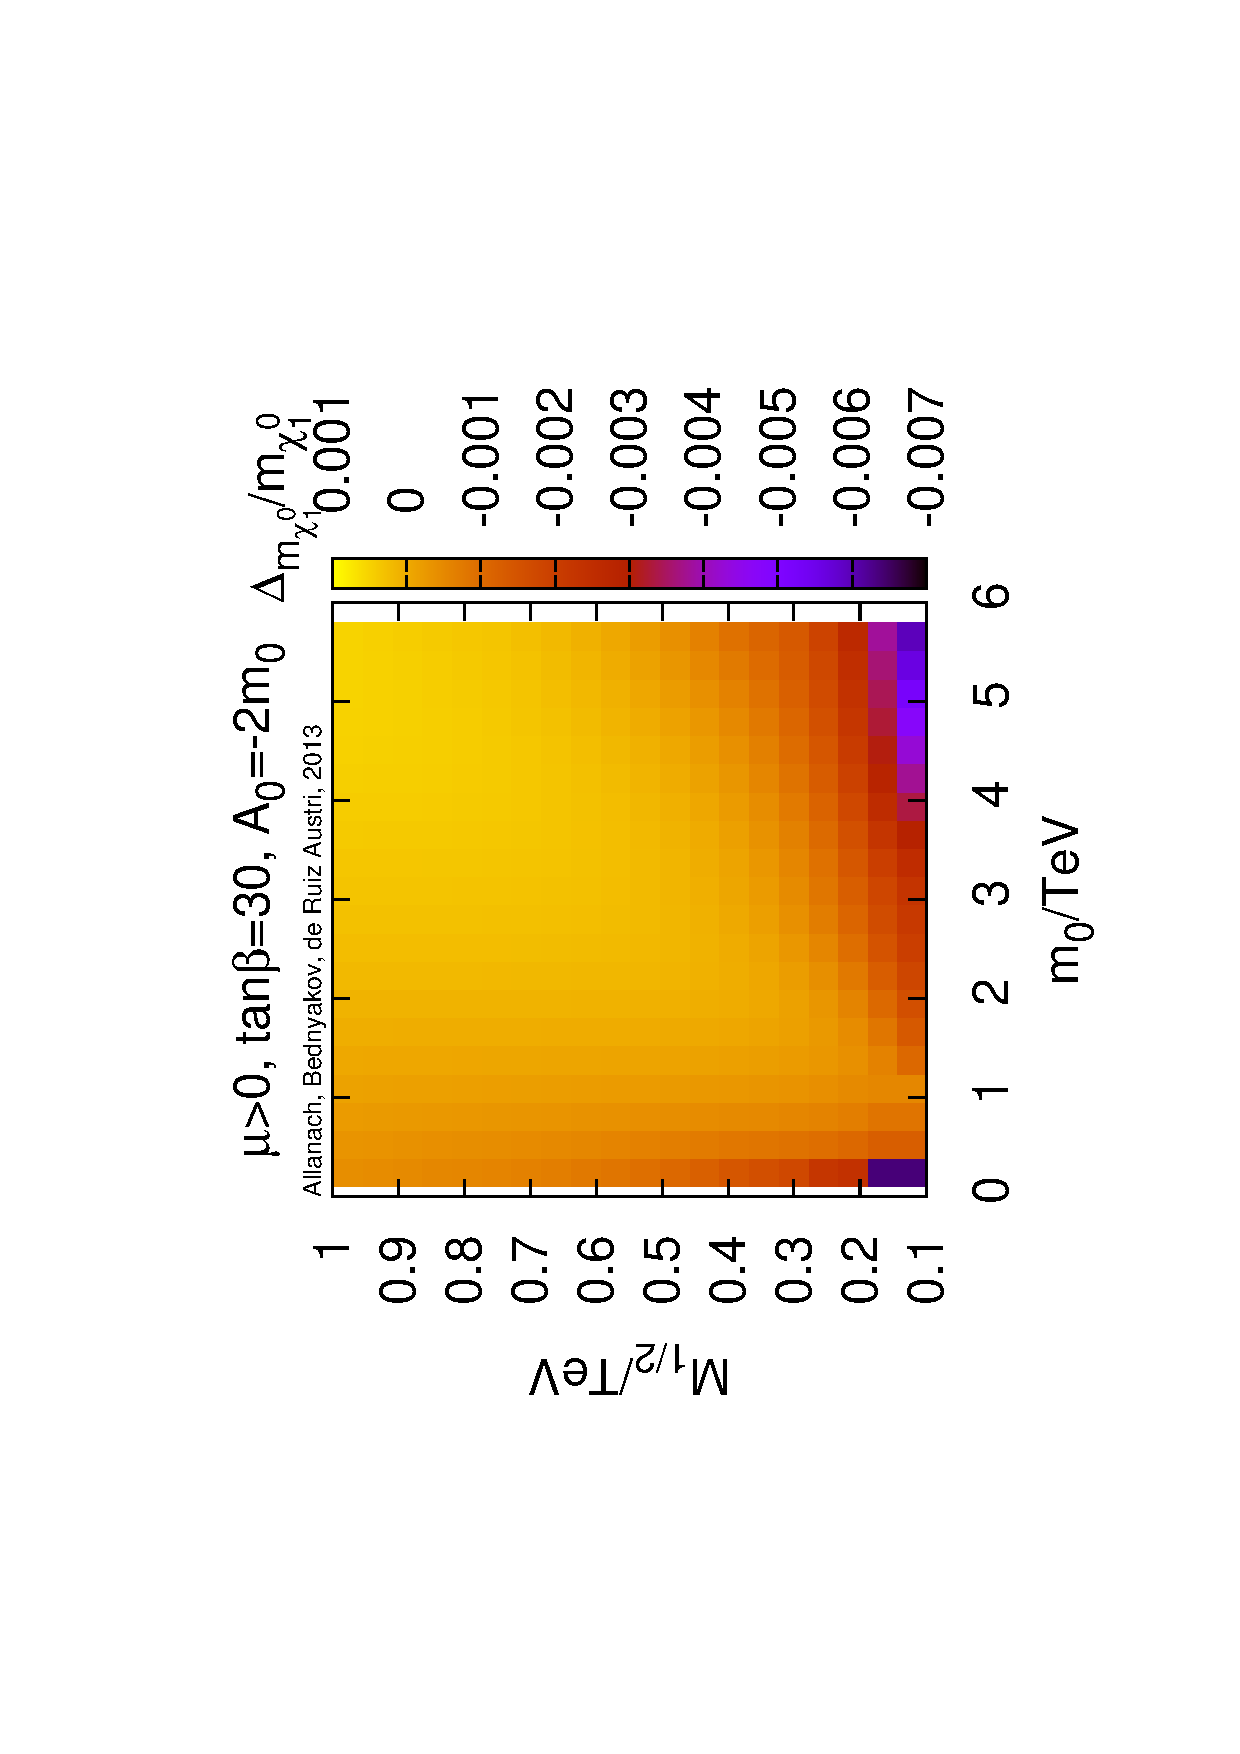
\includegraphics[angle=270,width=0.7\textwidth]{atlasScanMneut1}}
  \put(0.08,2.24){
\includegraphics[angle=270,width=0.45\textwidth]{atlasScanMneut12}}
  \put(-0.75,5.5){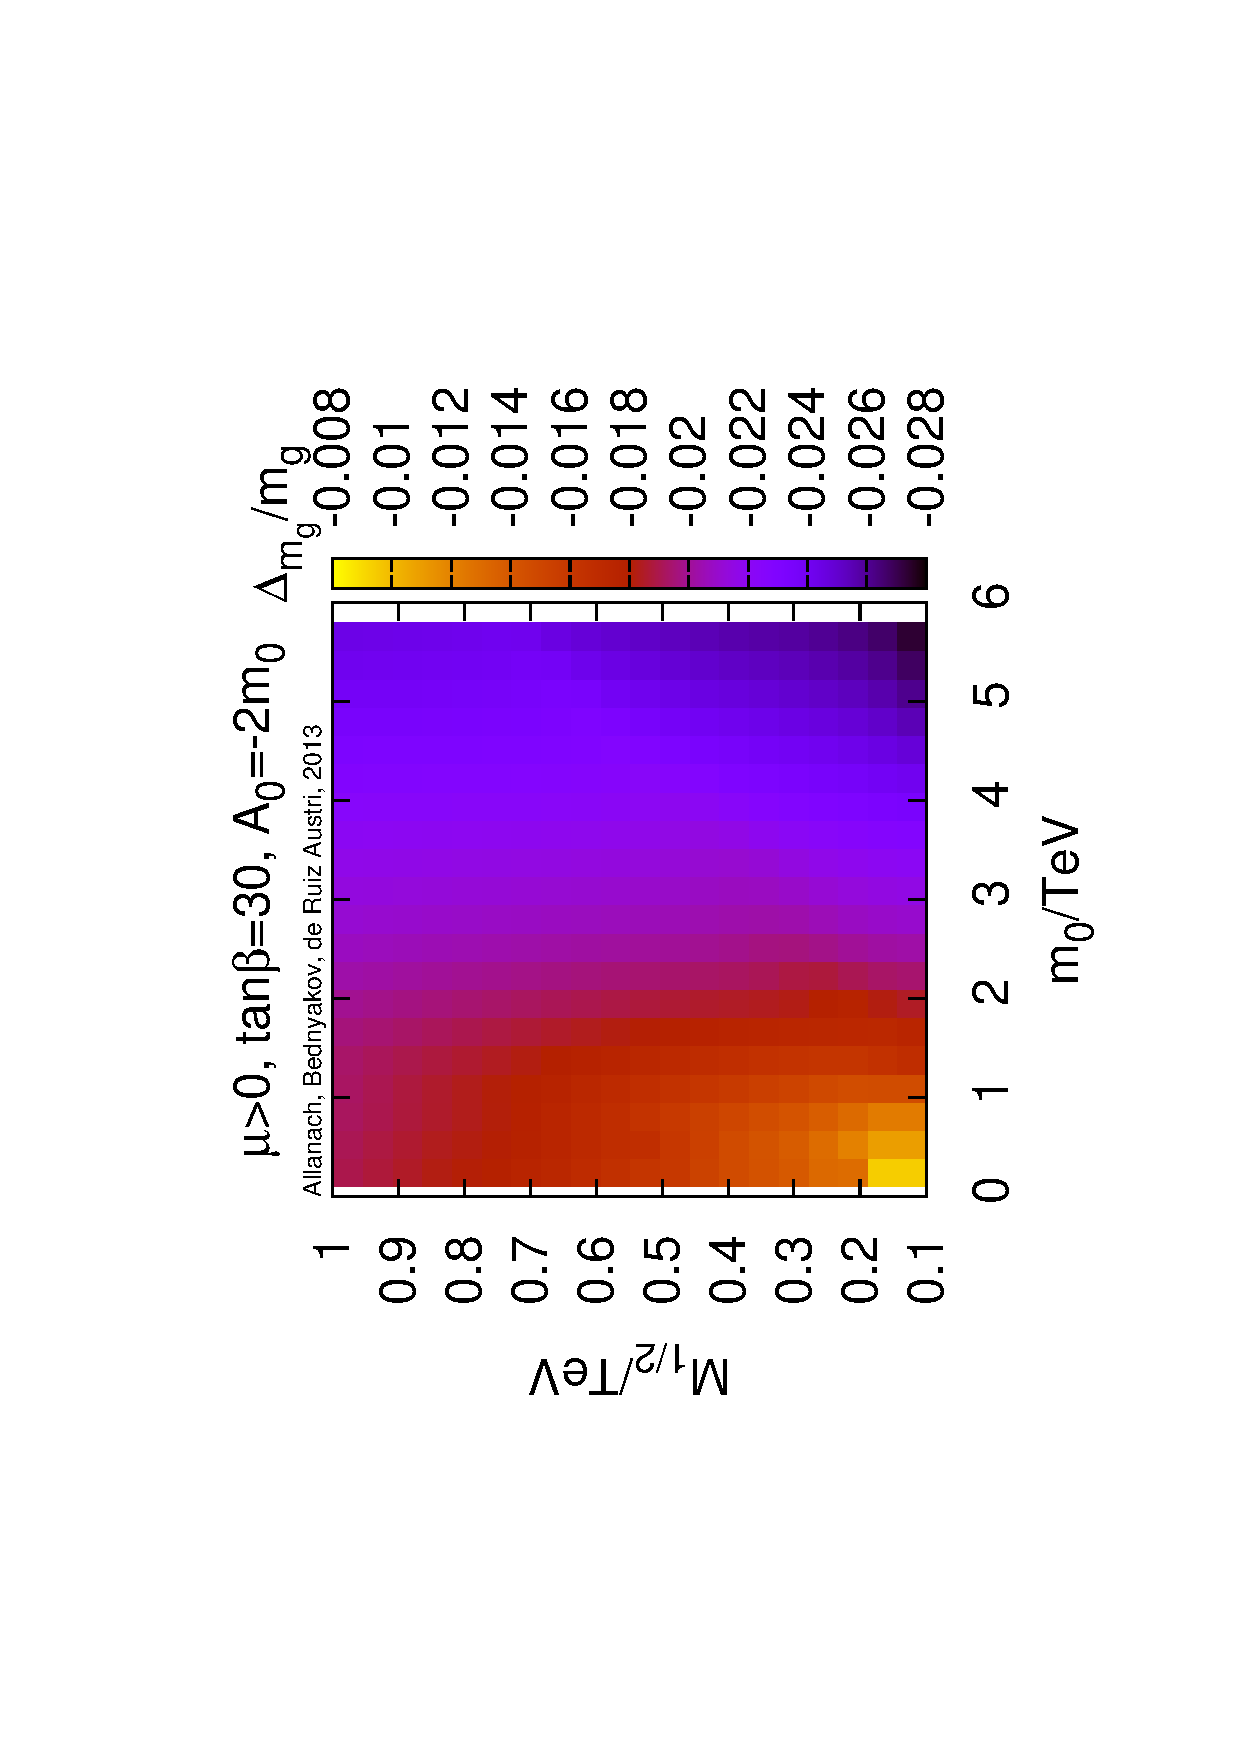
\includegraphics[angle=270,width=0.7\textwidth]{atlasScanMg}}
  \put(0.08,4.94){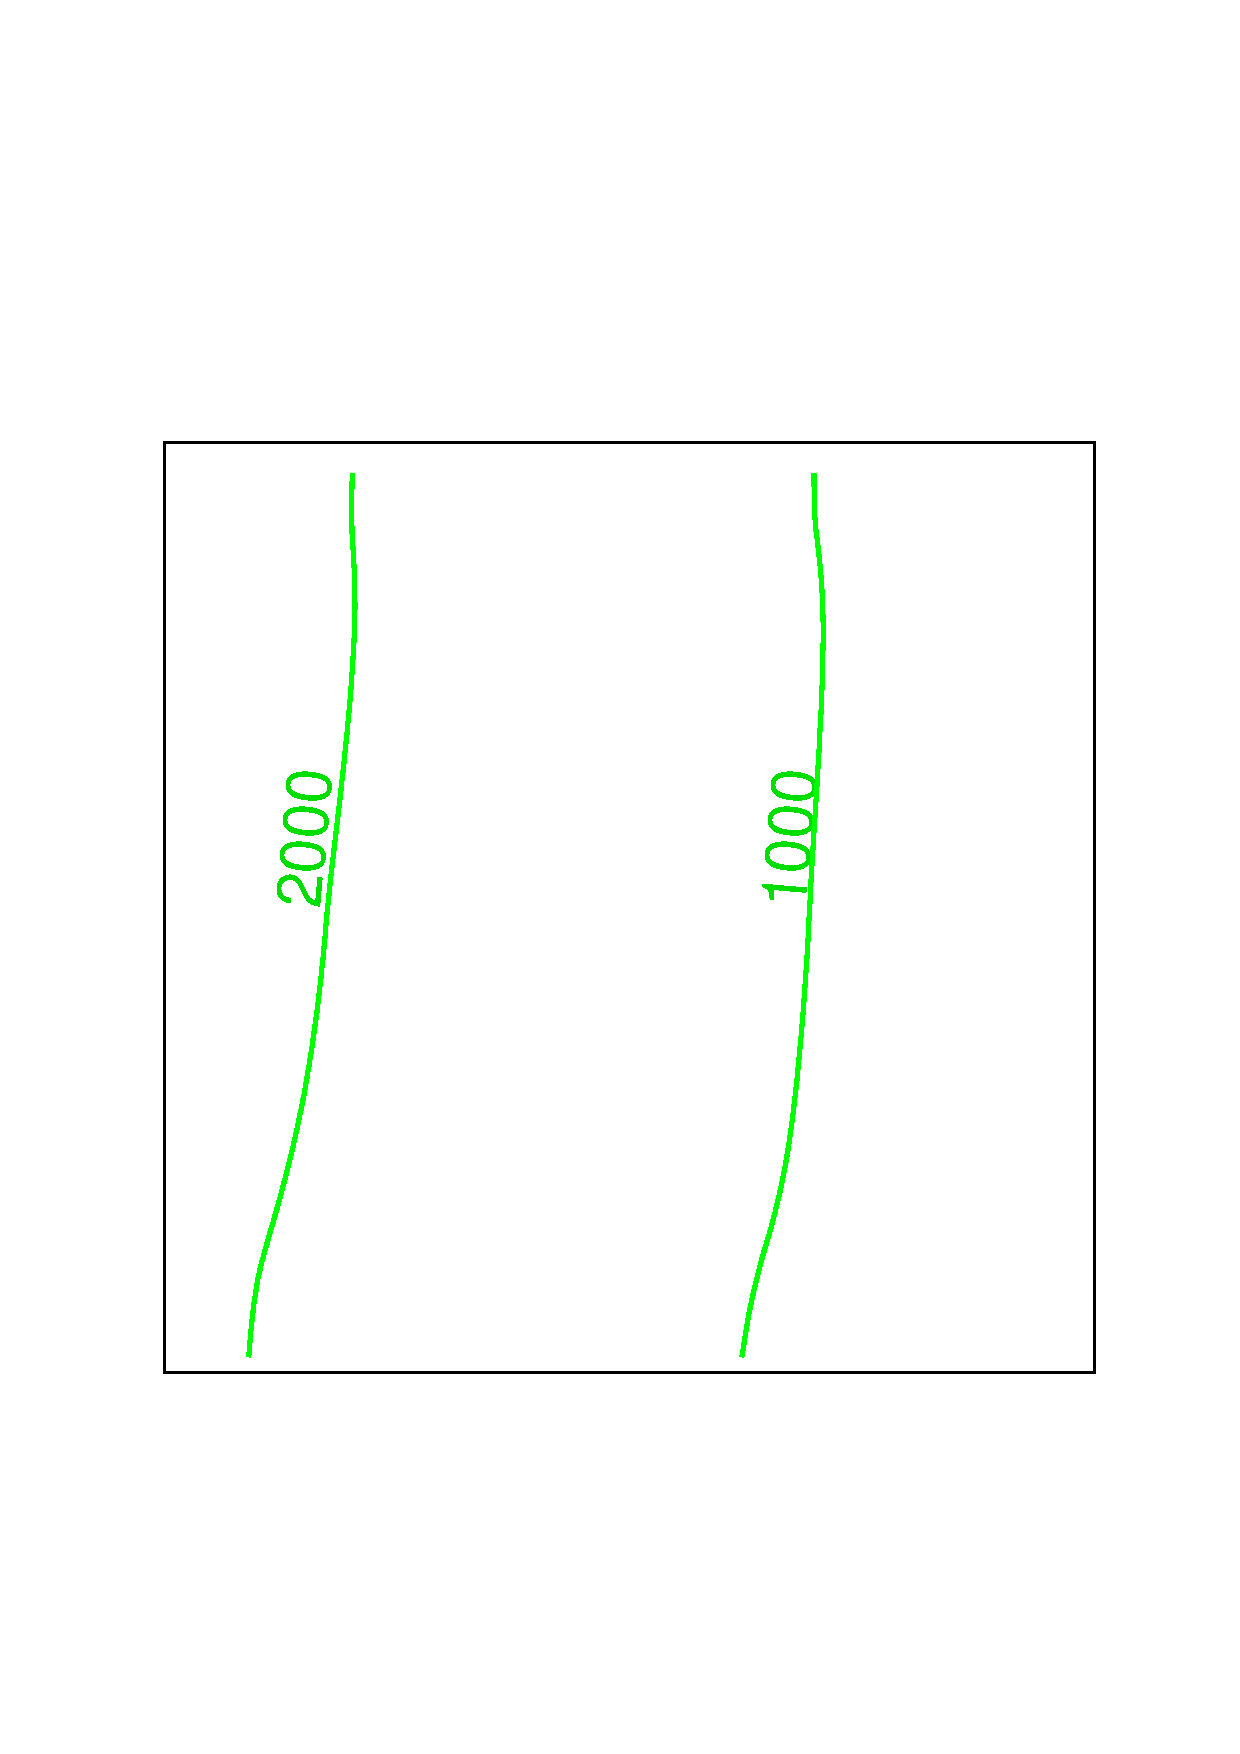
\includegraphics[angle=270,width=0.45\textwidth]{atlasScanMg2}}
  \put(2.4,2.8){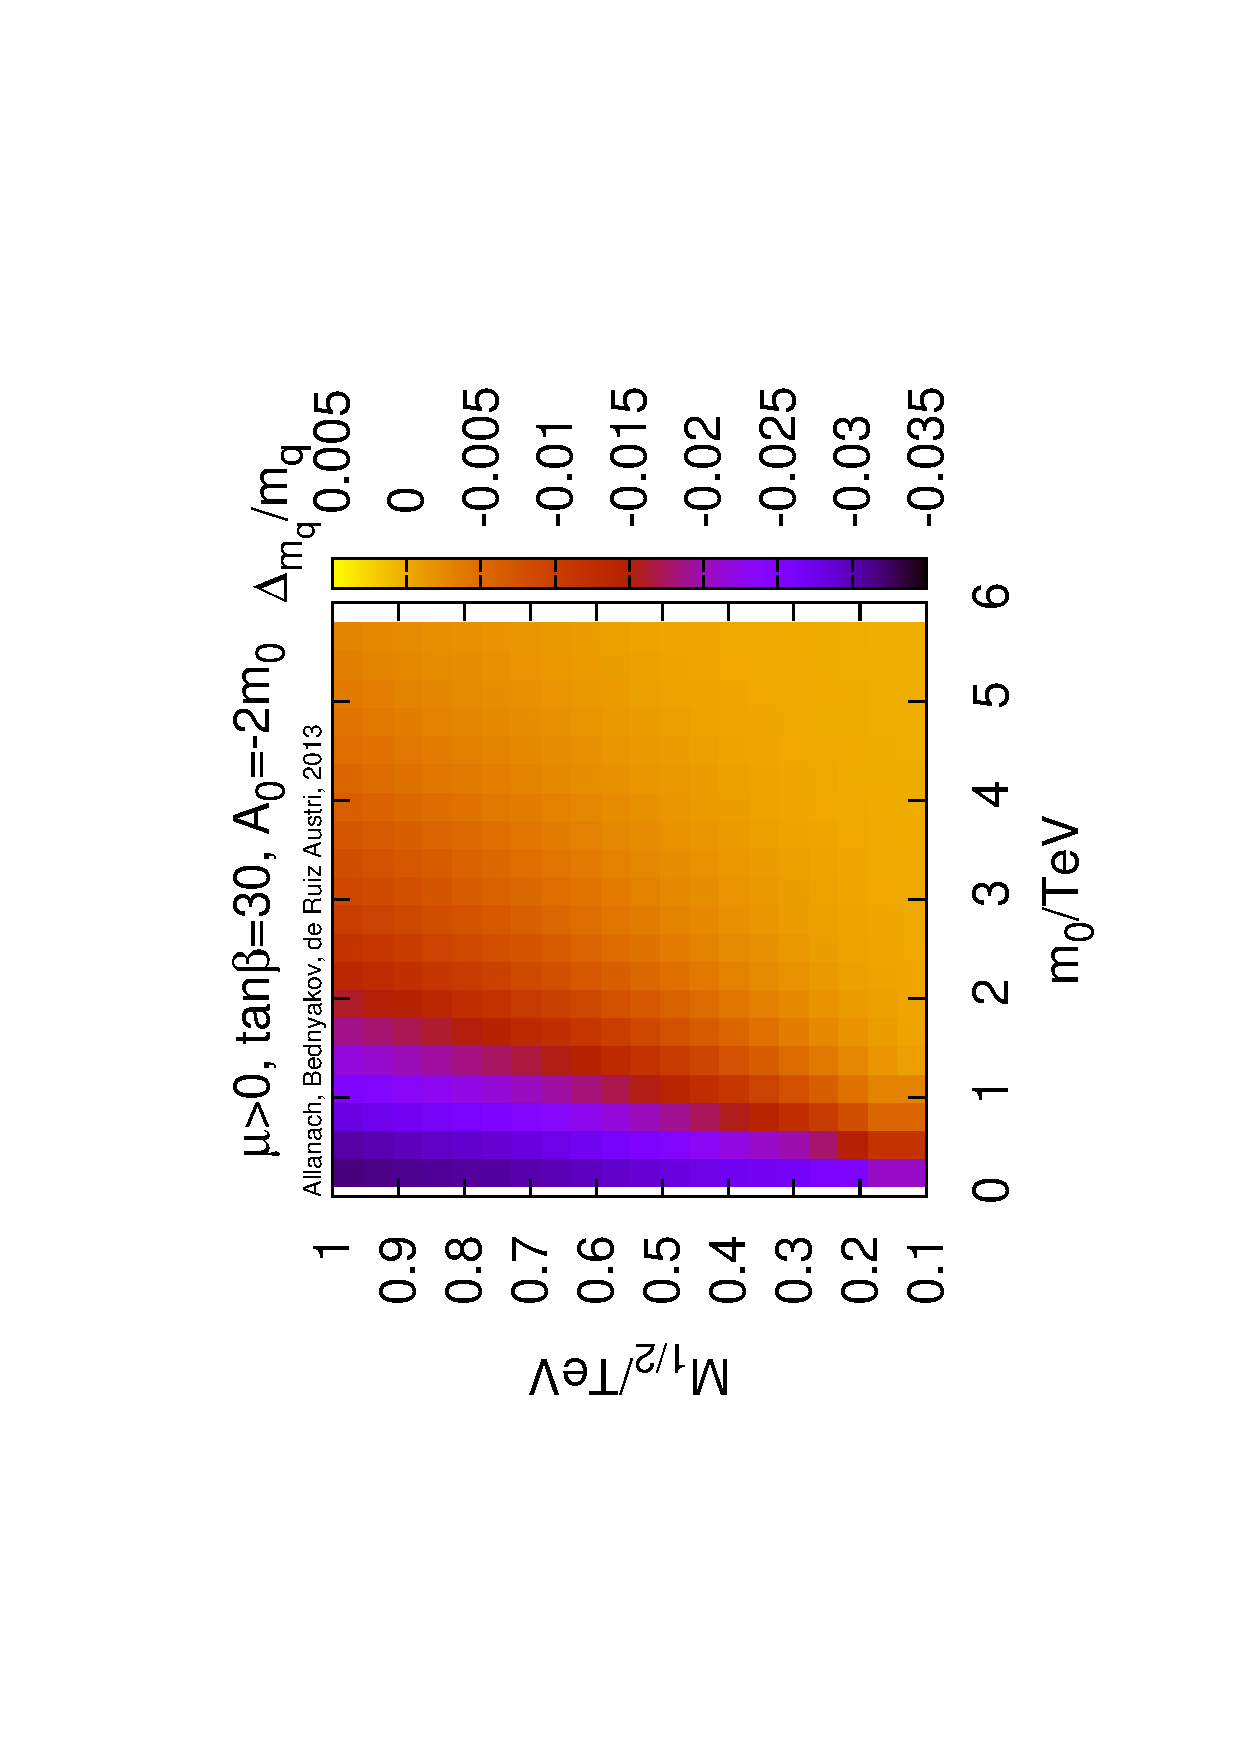
\includegraphics[angle=270,width=0.7\textwidth]{atlasScanMq}}
  \put(3.22,2.24){
\includegraphics[angle=270,width=0.45\textwidth]{atlasScanMq2}}
 \put(2.4,5.5){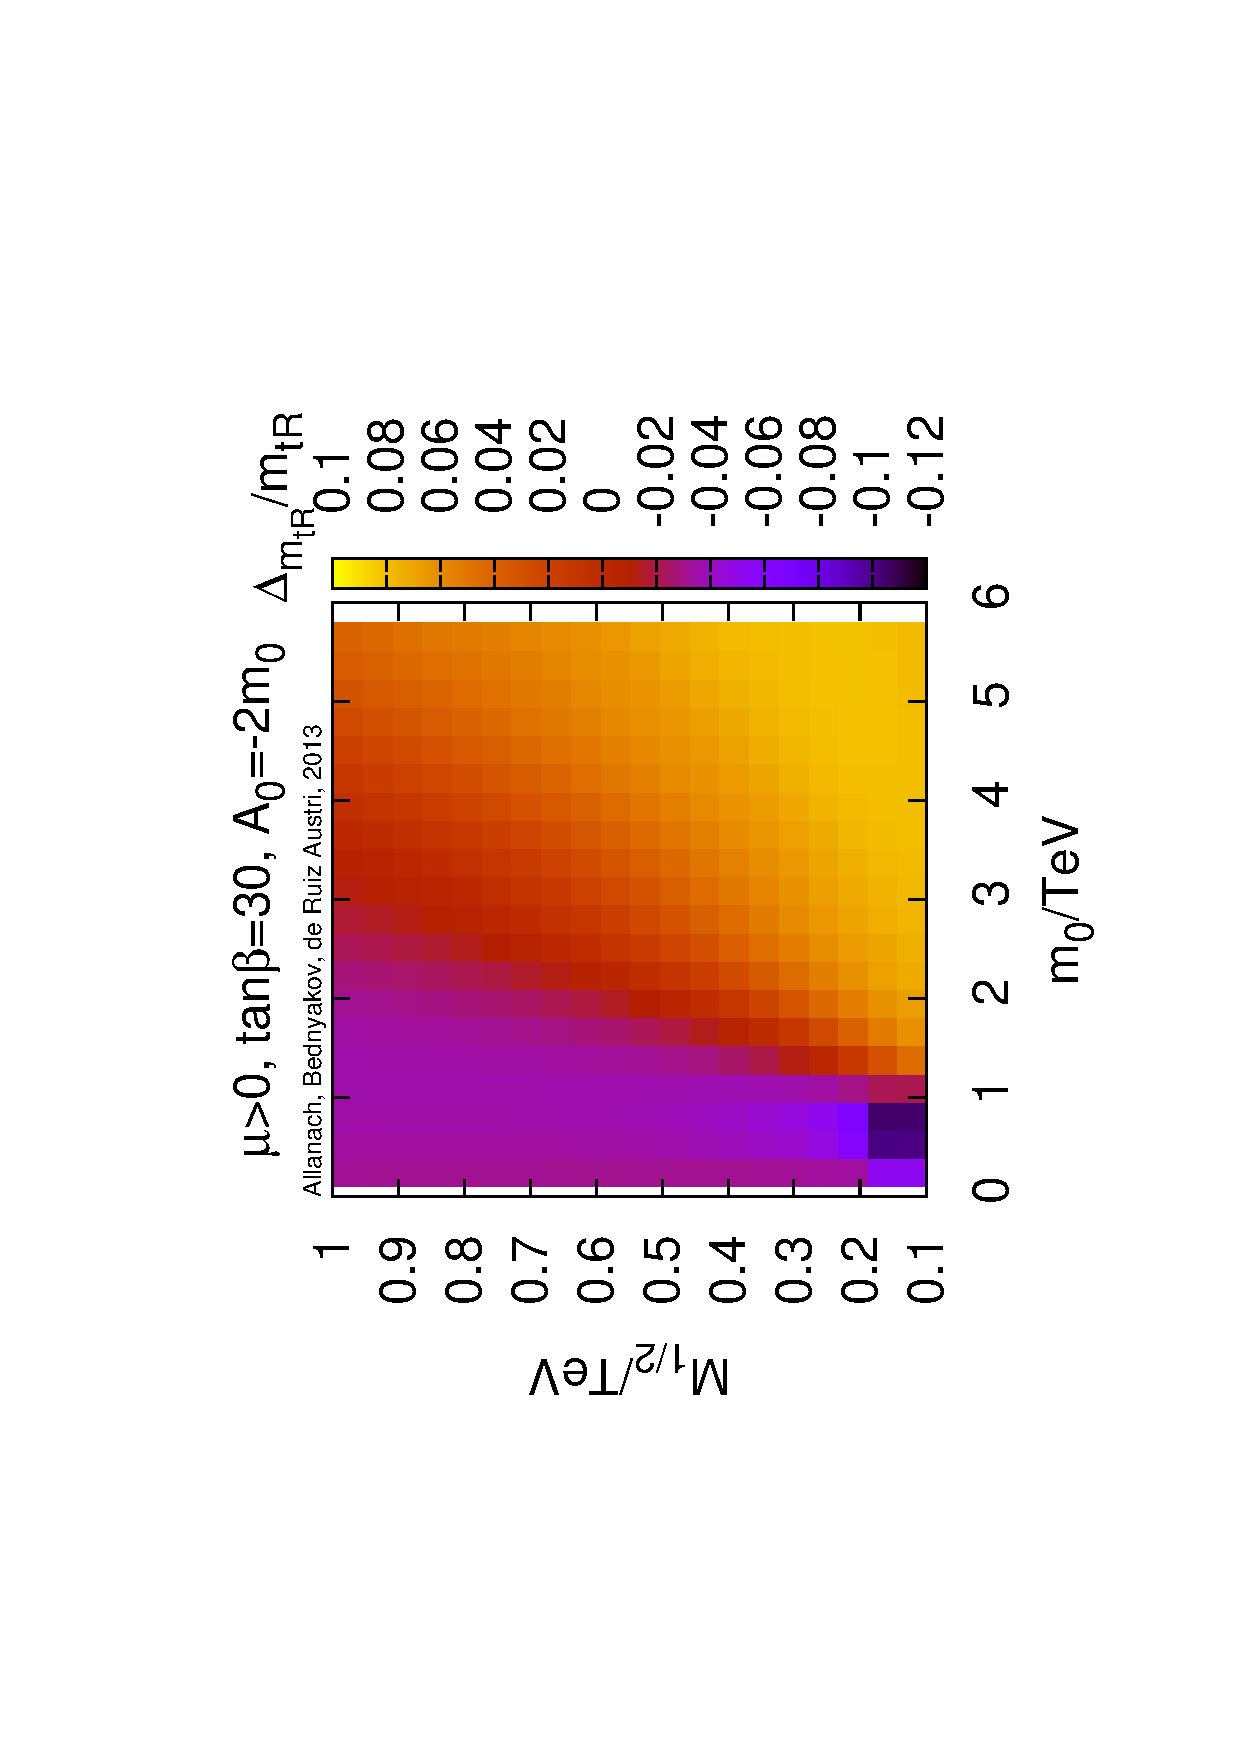
\includegraphics[angle=270,width=0.7\textwidth]{atlasScanMtR}}
  \put(3.22,4.94){
\includegraphics[angle=270,width=0.45\textwidth]{atlasScanMtR2}} 
  \put(-0.75,8.2){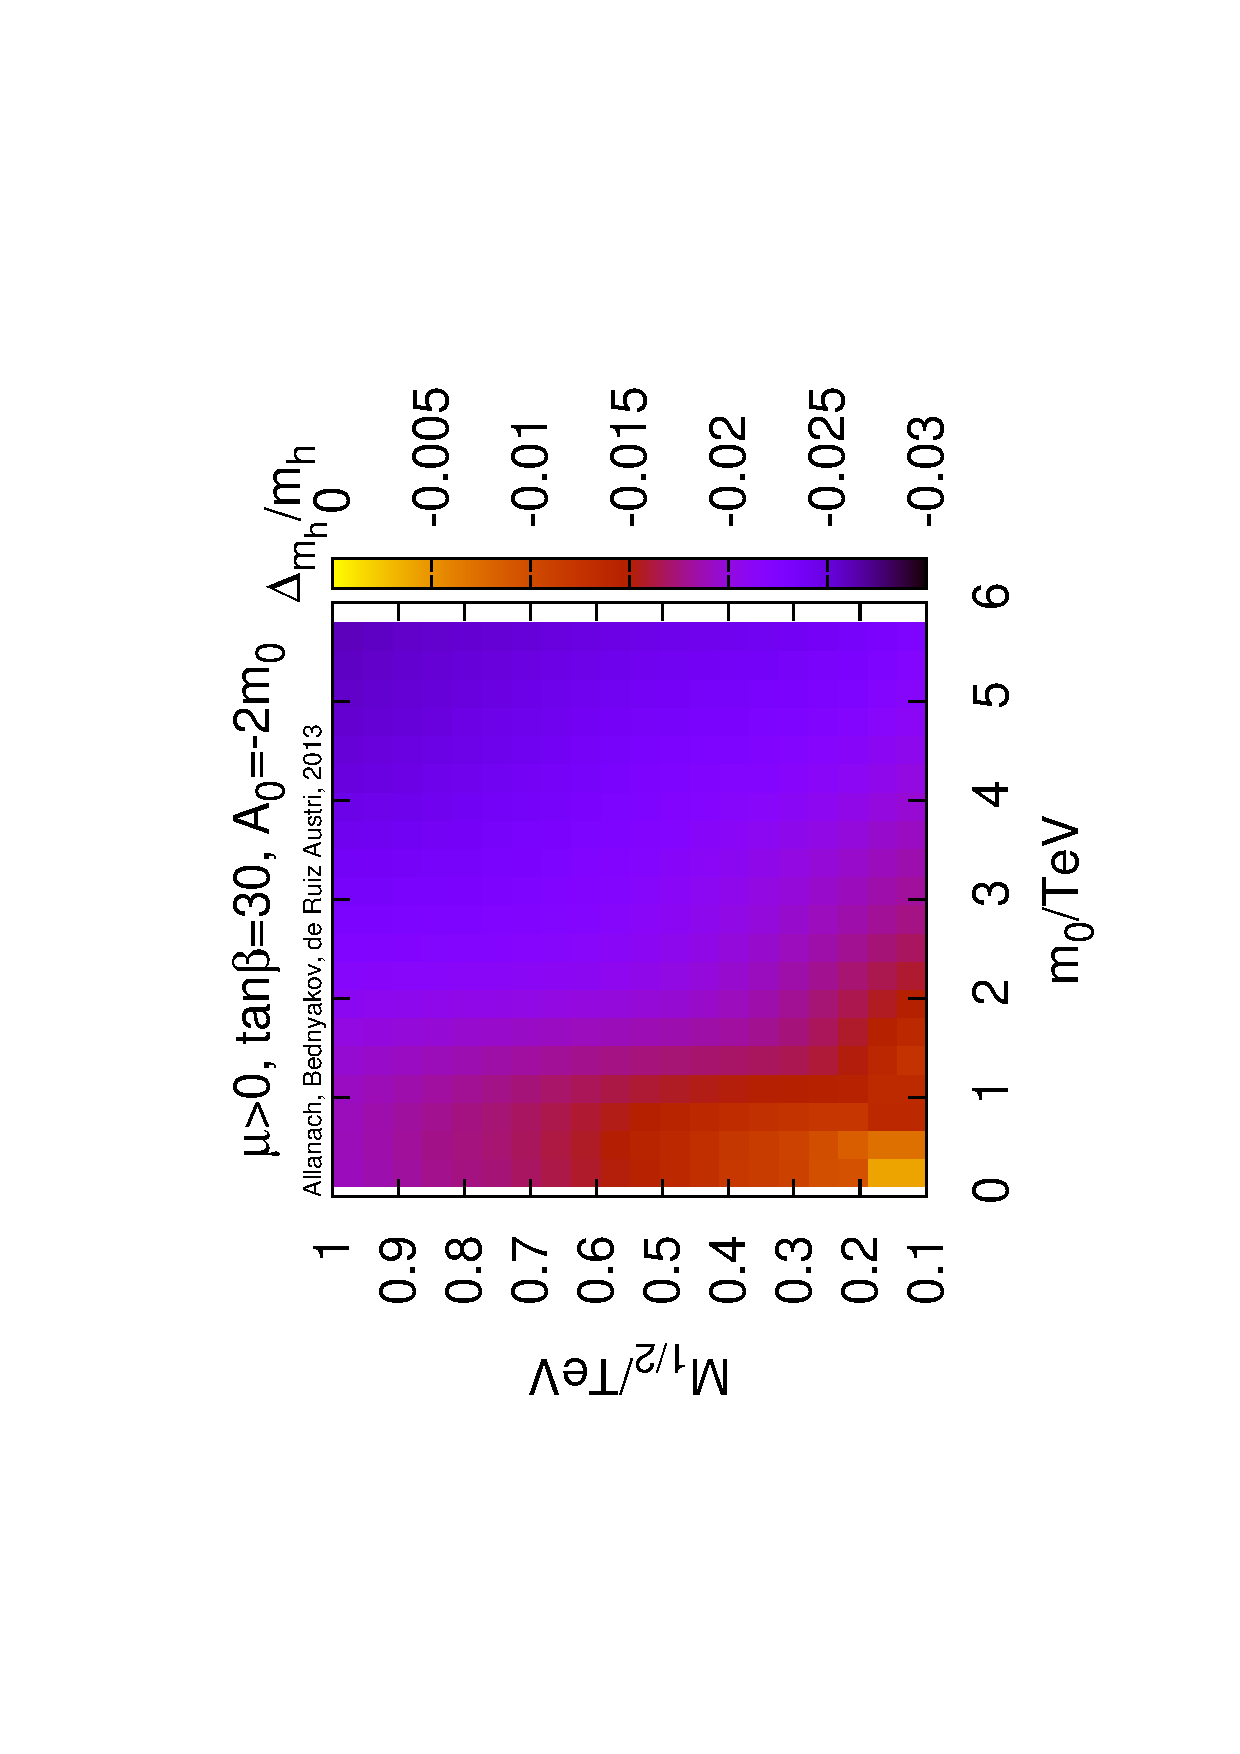
\includegraphics[angle=270,width=0.7\textwidth]{atlasScanMh}}
  \put(0.08,7.64){
\includegraphics[angle=270,width=0.45\textwidth]{atlasScanMh2}}
  \put(2.4,8.2){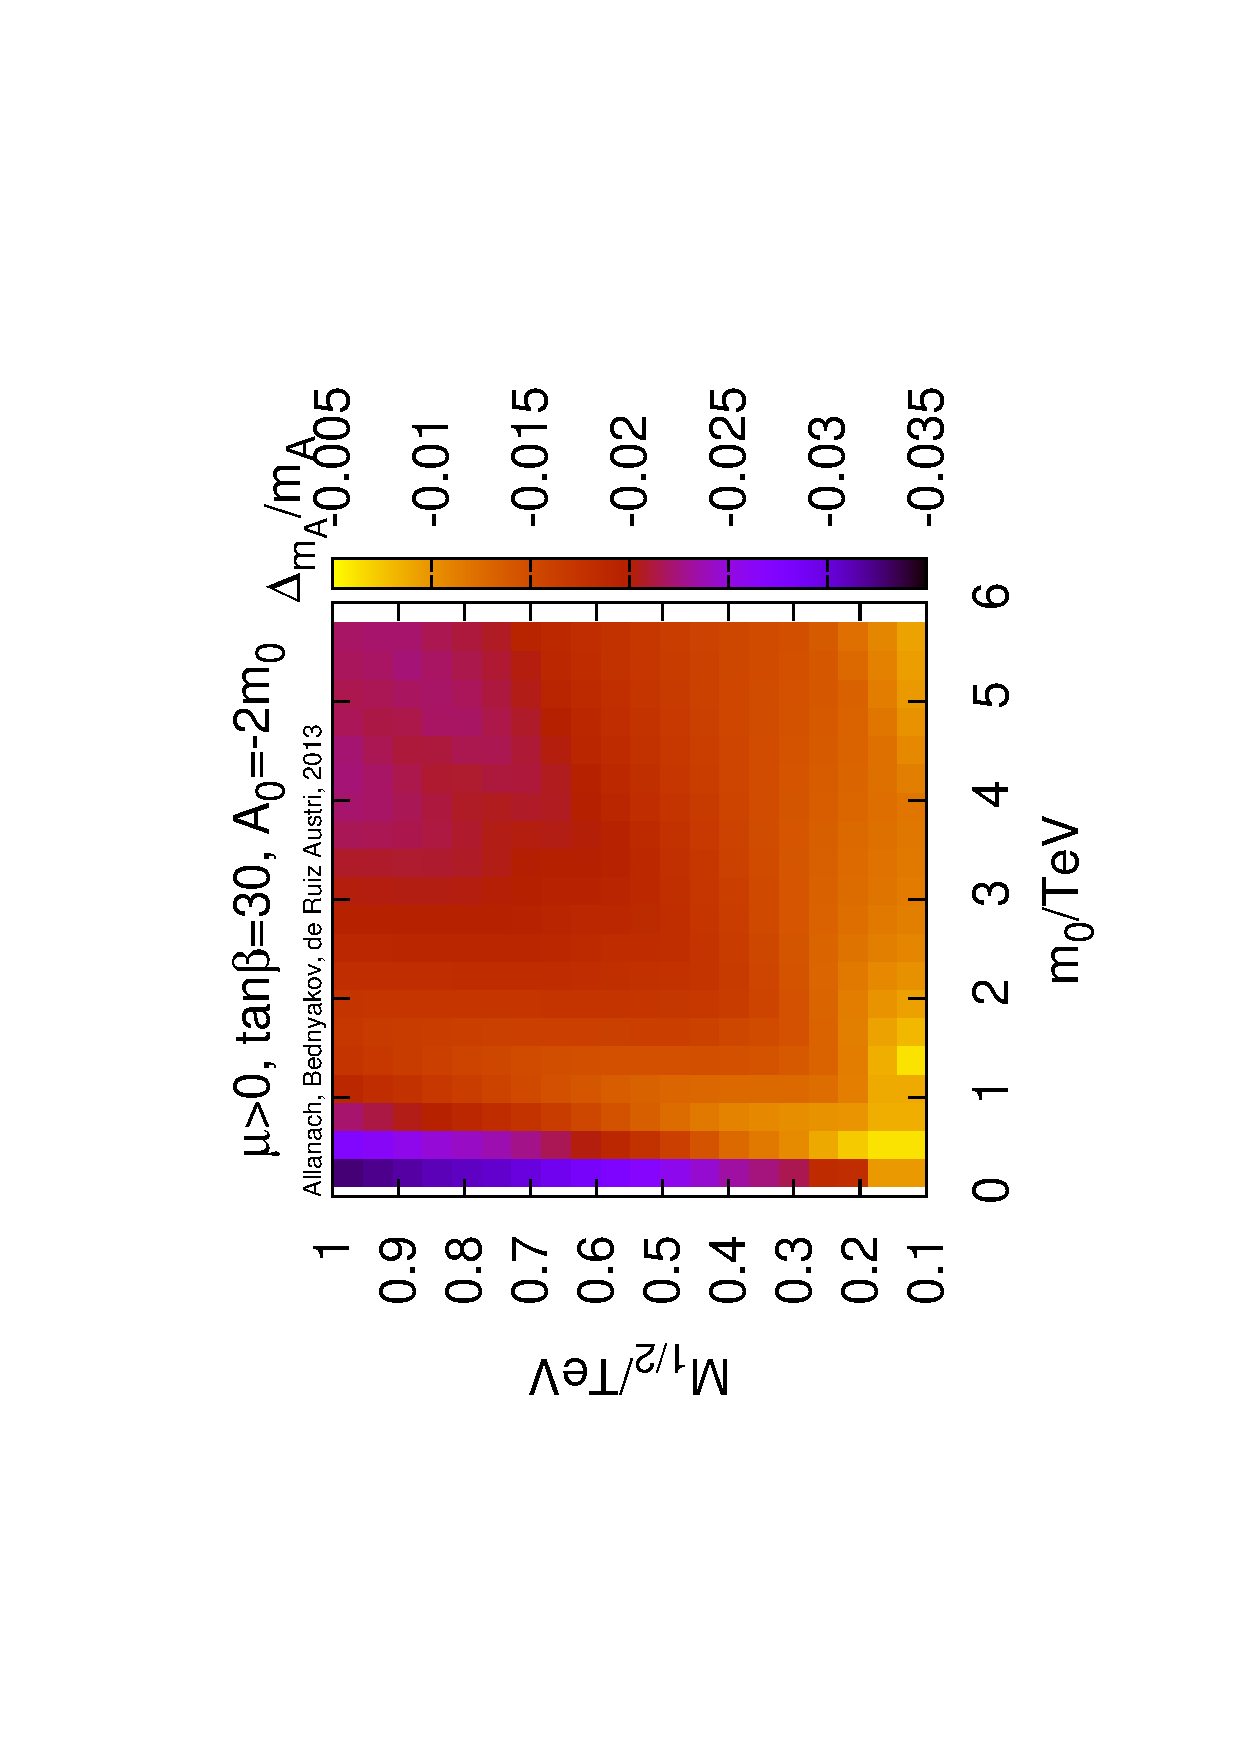
\includegraphics[angle=270,width=0.7\textwidth]{atlasScanMA}}
  \put(3.22,7.64){
\includegraphics[angle=270,width=0.45\textwidth]{atlasScanMA2}}
\put(0,7.8){(a)}
\put(3.2,7.8){(b)}
\put(0,5){(c)}
\put(3.2,5){(d)}
\put(0,2.2){(e)}
\put(3.2,2.2){(f)}
\end{picture}
\end{center}
\caption{\label{fig:dm} Relative effect of highest order terms (three-loop
  RGEs for gauge and Yukawa couplings and two-loop threshold corrections to
  third family fermion masses and $g_3$) on various
  particle pole masses in the CMSSM. The CMSSM 
  parameters coincide with the latest ATLAS
  CMSSM sparticle searches~\cite{}.
  Contours of iso-mass are overlayed on each
  figure, with each contour labelling the mass in GeV. Here, $m_g$ denotes the
gluino mass and $m_q$ the average squark mass from the first two generations. }
\end{figure}

\begin{figure}
\unitlength=1in
\begin{center}
\begin{picture}(3,3)
  \put(-0.75,2.8){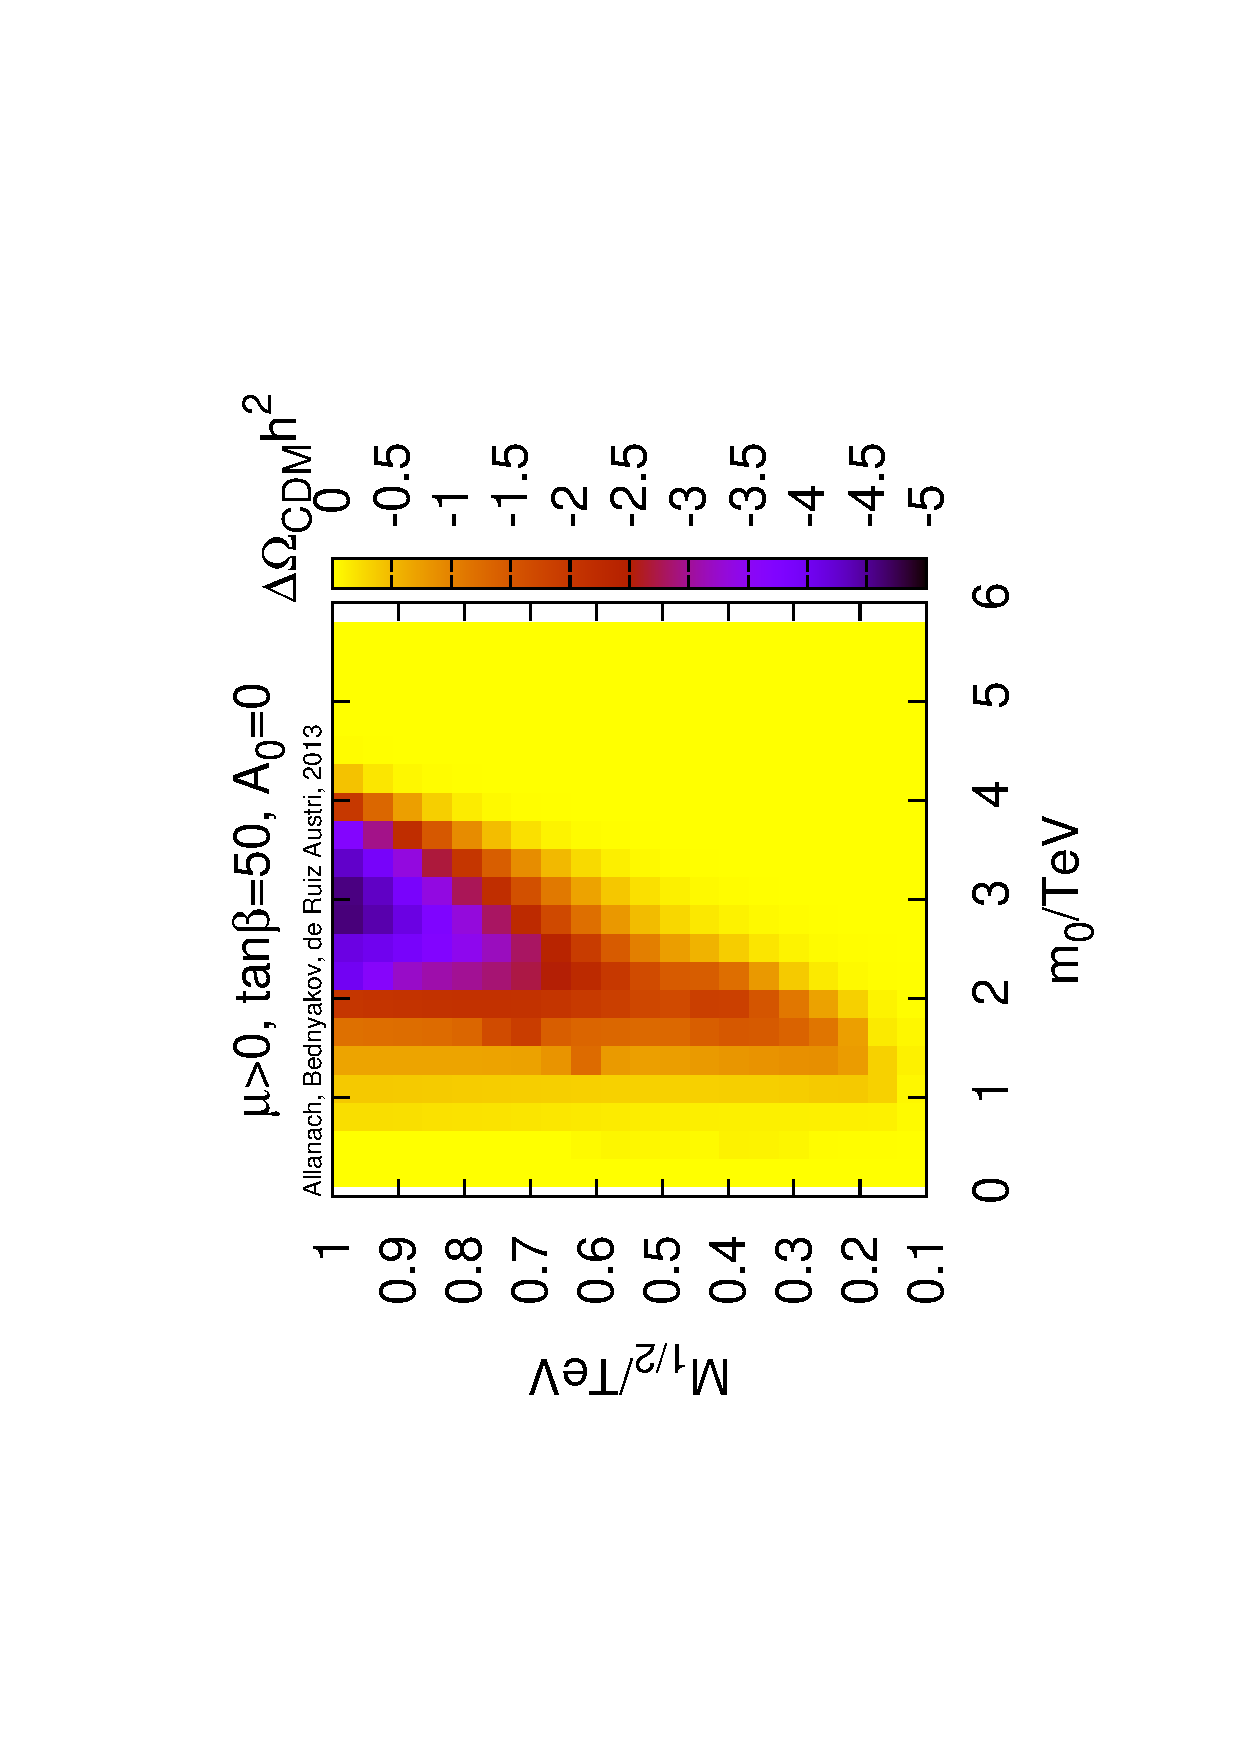
\includegraphics[angle=270,width=0.7\textwidth]{hiTbScanOm}}
  \put(0.08,2.24){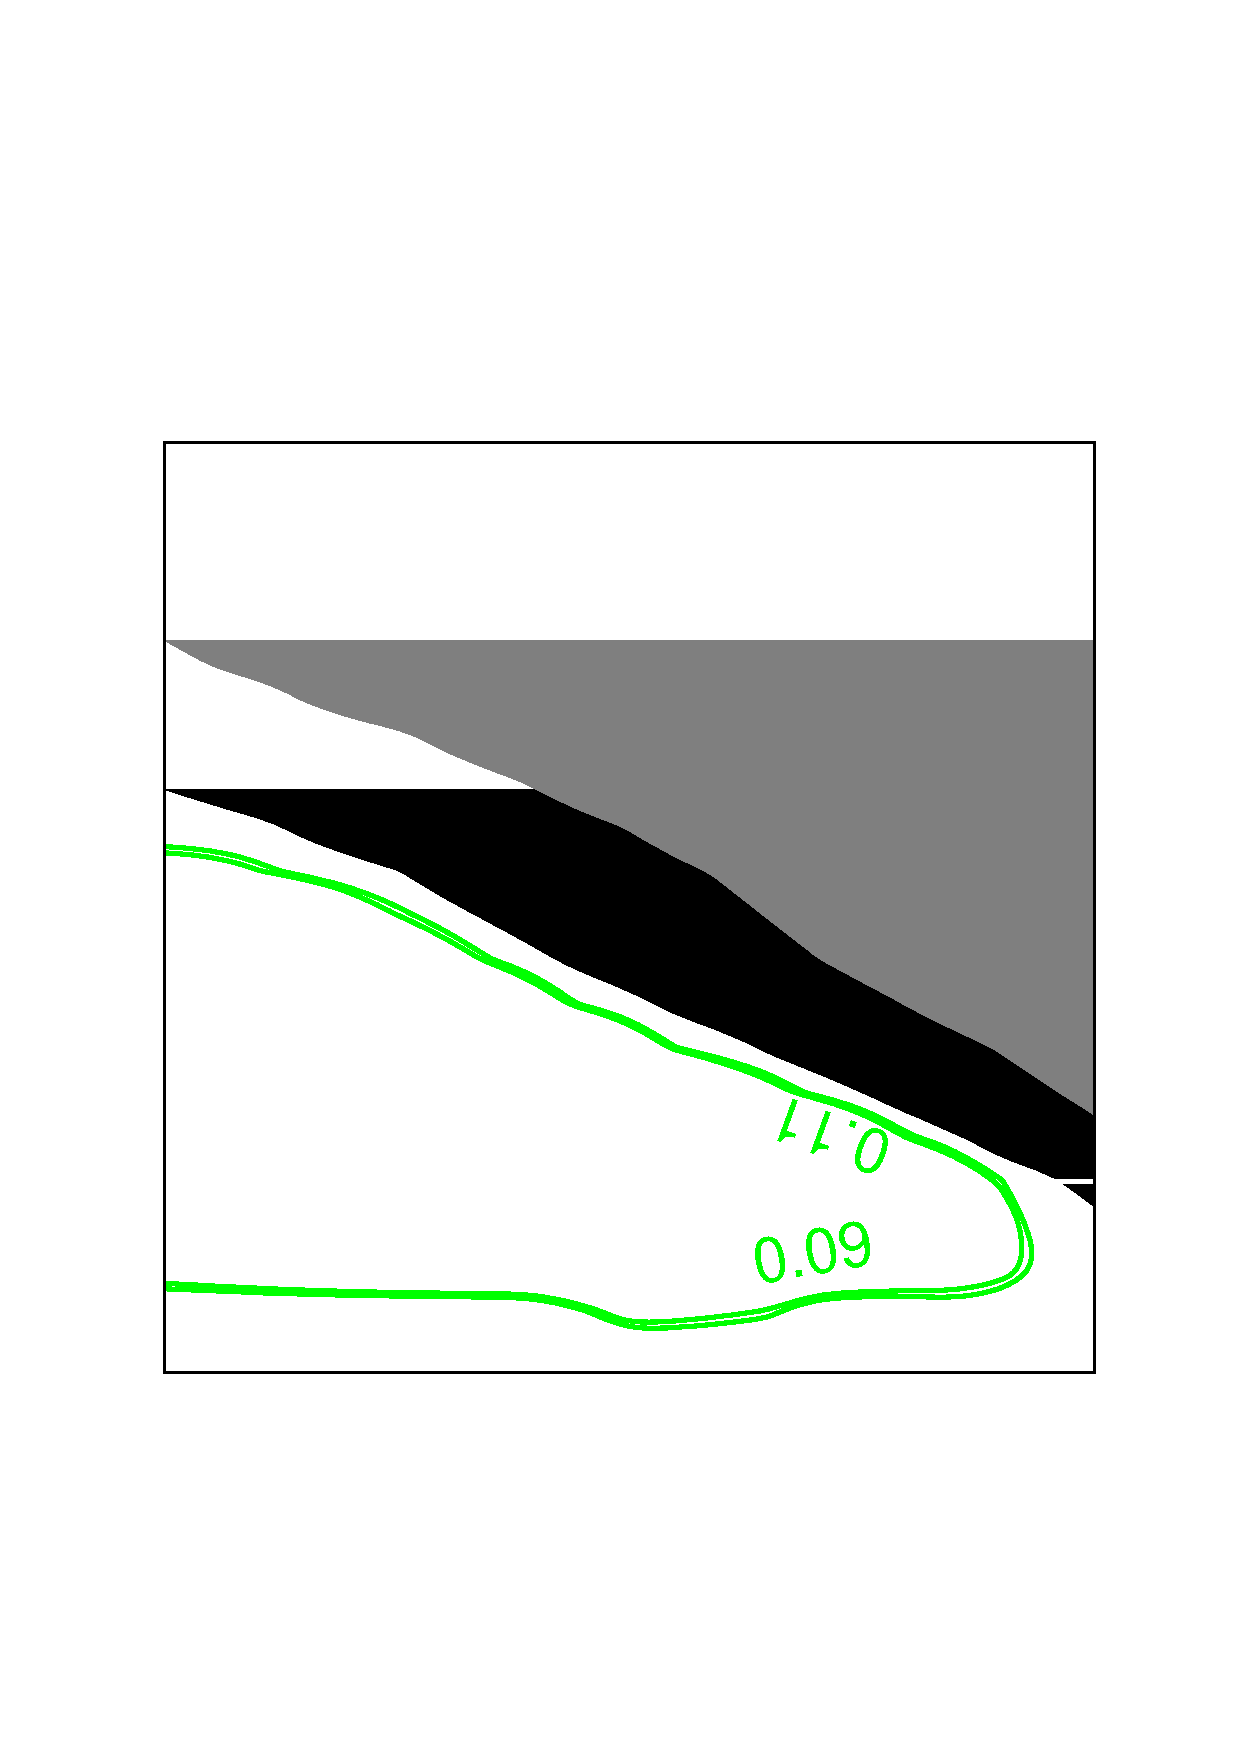
\includegraphics[angle=270,width=0.45\textwidth]{hiTbScanOm2}}
\end{picture}
\end{center}
\caption{\label{fig:dm} Effect of highest order terms (three-loop
  RGEs for gauge and Yukawa couplings and two-loop threshold corrections to
  third family fermion masses and $g_3$) on the predicted dark matter relic
  density in the CMSSM in a high $\tan \beta$ scenario. Contours of iso-relic
  density for the highest order prediction are overlayed. Also shown is the
  change in the position of the border of successful EWSB: the black region
  (and to the right) denotes the region for higher loop corrections, whereas
  the lighter one denotes the result of the standard \SOFTSUSY~calculation.}
\end{figure}


\begin{table}
\begin{center}
\begin{tabular}{|c|ccccccc|}\hline
quantity      & $m_h$  & $m_{\tilde g}$ & $m_{\chi_3^0}$  & $m_{\chi_4^0}$ &
$m_{\chi_2^\pm}$ & $m_{{\tilde d}_L,{\tilde s}_L}$ & $m_{{\tilde d}_R, {\tilde
    s}_R}$ \\ \hline
value         & 115.3  & 1087           & 2535          &  2574  & 2574 & 1058
&1027  \\
$\Delta$/$\%$ & -1.8  & -0.3         & -0.2        &  -0.1 & -0.1 & -0.1 &
-0.2\\ \hline
%
quantity & $g_3(M_{SUSY})$ & $Y_t(M_{SUSY})$ & $Y_b(M_{SUSY})$ &
$Y_\tau(M_{SUSY})$ & $\mu(M_{SUSY})$    &&\\ \hline
value &  1.036  & 0.836 & 0.128              &  0.097&2536 &&\\
$\Delta$/$\%$
& -1.0 & -1.9 & -1.8          &  -0.2&-0.2 &&\\
\hline
\end{tabular}
\end{center}
\caption{\label{tab:pmssm} Differences due to the highest order terms
  (three-loop 
  RGEs for gauge and Yukawa couplings and two-loop threshold corrections to
  third family fermion masses and $g_3$) on various quantities in the MSSM.
  We display quantities of with a relative error of greater than $10^{-3}$ for the
  parameter point pMSSM1.6~\cite{}. All masses are given in units of GeV, and
  $\Delta$ shows the relative change due to the highest order
  terms. $M_{SUSY}=\sqrt{m_{{\tilde t}_1} m_{{\tilde t}_2}}$ changes by less
    than 0.1 GeV due to the higher order effects.}
\end{table}

\section{Effect on Unification}


\section*{Acknowledgments}
This work has been partially supported by STFC 

\appendix

\section{Installation of the Increased Accuracy Mode}
\label{sec:install}

Two compilation options are added
\begin{itemize}
	\item[] \verb|--enable_three_loop_rge_compilation| - compile three-loop RGEs in the MSSM 
	\item[] \verb|--enable_full_susy_threshold_compilation| - compile additional two-loop threshold corrections to the third generation Yukawa couplings and the strong coupling constant 
\end{itemize}

Boolean variables that control the Increased Accuracy Mode at runtime
\begin{itemize}
	\item \verb|USE_THREE_LOOP_RGE = false|  - add three-loop contribution to MSSM RGE (corresponds to the \code{SOFTSUSY Block} parameter 19)
	\item \verb|USE_TWO_LOOP_THRESHOLD = false| - add two-loop threshold corrections to the third generation Yukawa couplings and the strong coupling constant
(corresponds to the \code{SOFTSUSY Block} parameter 20)
\end{itemize}

Additional variables that gives a finer control the Increased Accuracy Mode at runtime (with their default values)
\begin{itemize}
	\item \verb|double TWOLOOP_NUM_THRESH = 0.1|  - used in the iterative algorithm to prevent lengthy re-evaluation of two-loop thresholds 
		if the relative difference between the result obtained in current step and the  calcululated previously is less than \verb|TWOLOOP_NUM_THRESH| 
	\item \verb|boolean SOFTSUSY_TWOLOOP_blah = true| - control whether individual two-loop threshold corrections should be added (remove it or make a \verb|enum|?)
	\item \verb|boolean MB_DECOUPLING = false| - evaluate b-quark self-energies at $p=0$ in order to incorporate ``decoupling'' precedure (remove it?)
\end{itemize}


\section{Running \SOFTSUSY in the Increased Accuracy Mode} 
\label{sec:run}

\SOFTSUSY~produces an executable called \code{softpoint.x}. For the calculation
of the spectrum of single points in parameter space, we recommend the
SUSY Les Houches Accord 2 (SLHA2)~\cite{Allanach:2008qq}  input/output
option. The user must provide a file (e.g.\ the example file included
in the \SOFTSUSY~distribution
\code{rpvHouchesInput}), that specifies the model dependent input
parameters. The program may then be run with
\small
\begin{verbatim}
 ./softpoint.x leshouches < inOutFiles/lesHouchesInput
\end{verbatim}
\normalsize

One can change whether the 3-loop RGE corrections are switched on with
\code{SOFTSUSY Block} parameter 19, whereas the 2-loop third family and $g_3$
threshold corrections 
are switched on with \code{SOFTSUSY Block} parameter 20 in the SLHA2 input file:
\small
\begin{verbatim}
Block SOFTSUSY               # Optional SOFTSUSY-specific parameters
   19   1.000000000e+00      # Include 3-loop RGE terms (0 to disable)
   20   1.000000000e+00      # Include 2-loop thresholds (0 to disable)
\end{verbatim}
\normalsize


\begin{thebibliography}{10}
\bibitem{Aad:2013wta}
  G.~Aad {\it et al.}  [ATLAS Collaboration],
  %``Search for new phenomena in final states with large jet multiplicities and missing transverse momentum at $\sqrt{s}=8$ TeV proton-proton collisions using the ATLAS experiment,''
  JHEP {\bf 1310} (2013) 130
  [arXiv:1308.1841 [hep-ex]].
  %%CITATION = ARXIV:1308.1841;%%
  %10 citations counted in INSPIRE as of 06 Nov 2013
%\cite{Aad:2012tfa}
\bibitem{CMSspart}
S.~Chatrchyan {\it et al.} [CMS Collaboration], (2013) CMS-PAS-SUS-13-012
    %\cite{Allanach:2008zn}
\bibitem{Allanach:2008zn}
  B.~C.~Allanach,
  %``SUSY Predictions and SUSY Tools at the LHC,''
  Eur.\ Phys.\ J.\ C {\bf 59} (2009) 427
  [arXiv:0805.2088 [hep-ph]].
  %%CITATION = ARXIV:0805.2088;%%
  %13 citations counted in INSPIRE as of 06 Nov 2013

  \bibitem{Baer:1993ae}
H.~Baer, F.~E. Paige, S.~D. Protopopescu and X.~Tata, 
%{\it {Simulating
%  Supersymmetry with ISAJET 7.0 / ISASUSY 1.0}},
[hep-ph/9305342].
%%CITATION = HEP-PH/9305342;%%
%\cite{Allanach:2001kg}
\bibitem{Allanach:2001kg} 
  B.~C.~Allanach,
  %``SOFTSUSY: a program for calculating supersymmetric spectra,''
  Comput.\ Phys.\ Commun.\  {\bf 143}, 305 (2002)
  [hep-ph/0104145].
  %%CITATION = HEP-PH/0104145;%%
  %716 citations counted in INSPIRE as of 20 Sep 2013

\bibitem{Porod:2003um}
W.~Porod, 
%{\it {SPheno, a program for calculating supersymmetric spectra, SUSY
%  particle decays and SUSY particle production at e+ e- colliders}},  
  Comput.\ Phys.\ Commun. {\bf 153} (2003) 275--315
  [hep-ph/0301101].
%%CITATION = HEP-PH/0301101;%%
\bibitem{Chowdhury:2011zr}
D.~Chowdhury, R.~Garani and S.~K. Vempati, 
%{\it {SUSEFLAV: Program for
%  supersymmetric mass spectra with seesaw mechanism and rare lepton flavor
%  violating decays}},  
Comput.\ Phys.\ Commun. {\bf 184} (2013) 899--918
  [arXiv:1109.3551 [hep-ph]].
%%CITATION = ARXIV:1109.3551;%%

\bibitem{Djouadi:2002ze}
A.~Djouadi, J.-L. Kneur and G.~Moultaka, 
%{\it {SuSpect: A Fortran code for the
%  supersymmetric and Higgs particle spectrum in the MSSM}},  
  Comput.\ Phys.\ Commun. {\bf 176} (2007) 426--455
  [hep-ph/0211331].
%%CITATION = HEP-PH/0211331;%%
%\cite{Djouadi:2013lra}

%\cite{Skands:2003cj}
\bibitem{Skands:2003cj}
  P.~Z.~Skands, B.~C.~Allanach, H.~Baer, C.~Balazs, G.~Belanger, F.~Boudjema, A.~Djouadi and R.~Godbole {\it et al.},
  %``SUSY Les Houches accord: Interfacing SUSY spectrum calculators, decay packages, and event generators,''
  JHEP {\bf 0407} (2004) 036
  [hep-ph/0311123].
  %%CITATION = HEP-PH/0311123;%%
  %380 citations counted in INSPIRE as of 07 Nov 2013
\bibitem{Aad:2012tfa}
  G.~Aad {\it et al.}  [ATLAS Collaboration],
  %``Observation of a new particle in the search for the Standard Model Higgs boson with the ATLAS detector at the LHC,''
  Phys.\ Lett.\ B {\bf 716} (2012) 1
  [arXiv:1207.7214 [hep-ex]].
  %%CITATION = ARXIV:1207.7214;%%
  %1868 citations counted in INSPIRE as of 06 Nov 2013
%\cite{Chatrchyan:2012ufa}
\bibitem{Chatrchyan:2012ufa}
  S.~Chatrchyan {\it et al.}  [CMS Collaboration],
  %``Observation of a new boson at a mass of 125 GeV with the CMS experiment at the LHC,''
  Phys.\ Lett.\ B {\bf 716} (2012) 30
  [arXiv:1207.7235 [hep-ex]].
  %%CITATION = ARXIV:1207.7235;%%
  %1848 citations counted in INSPIRE as of 06 Nov 2013

\bibitem{ATLAS-CONF-2013-014}
G.~Aad {\it et al.}  [ATLAS Collaboration],
ATLAS-CONF-2013-014, talk delivered at 48th Rencontres de Moriond on Electroweak Interactions and Unified Theories, La Thuile, Italy, 2 - 9 Mar 2013.


\bibitem{Djouadi:2013lra}
  A.~Djouadi,
  %``Implications of the Higgs discovery for the MSSM,''
  arXiv:1311.0720 [hep-ph].
  %%CITATION = ARXIV:1311.0720;%%

\bibitem{Barbieri:1998uv}
  R.~Barbieri and A.~Strumia,
  %``About the fine tuning price of LEP,''
  Phys.\ Lett.\ B {\bf 433} (1998) 63
  [hep-ph/9801353].
  %%CITATION = HEP-PH/9801353;%%
  %94 citations counted in INSPIRE as of 07 Nov 2013

%\cite{Arbey:2011ab}
\bibitem{Arbey:2011ab}
  A.~Arbey, M.~Battaglia, A.~Djouadi, F.~Mahmoudi and J.~Quevillon,
  %``Implications of a 125 GeV Higgs for supersymmetric models,''
  Phys.\ Lett.\ B {\bf 708} (2012) 162
  [arXiv:1112.3028 [hep-ph]].
  %%CITATION = ARXIV:1112.3028;%%
  %188 citations counted in INSPIRE as of 07 Nov 2013
%\cite{Delgado:2010uj}
\bibitem{Delgado:2010uj}
  A.~Delgado, C.~Kolda, J.~P.~Olson and A.~de la Puente,
  %``Solving the Little Hierarchy Problem with a Singlet and Explicit $\mu$ Terms,''
  Phys.\ Rev.\ Lett.\  {\bf 105} (2010) 091802
  [arXiv:1005.1282 [hep-ph]].
  %%CITATION = ARXIV:1005.1282;%%
  %38 citations counted in INSPIRE as of 07 Nov 2013
\bibitem{Ellwanger:2011mu}
  U.~Ellwanger, G.~Espitalier-Noel and C.~Hugonie,
  %``Naturalness and Fine Tuning in the NMSSM: Implications of Early LHC Results,''
  JHEP {\bf 1109} (2011) 105
  [arXiv:1107.2472 [hep-ph]].
  %%CITATION = ARXIV:1107.2472;%%
  %42 citations counted in INSPIRE as of 07 Nov 2013
%\cite{King:2012tr}
\bibitem{King:2012tr}
  S.~F.~King, M.~Mühlleitner, R.~Nevzorov and K.~Walz,
  %``Natural NMSSM Higgs Bosons,''
  Nucl.\ Phys.\ B {\bf 870} (2013) 323
  [arXiv:1211.5074 [hep-ph]].
  %%CITATION = ARXIV:1211.5074;%%
  %36 citations counted in INSPIRE as of 07 Nov 2013
%\cite{Perelstein:2012qg}
\bibitem{Perelstein:2012qg}
  M.~Perelstein and B.~Shakya,
  %``XENON100 Implications for Naturalness in the MSSM, NMSSM and lambda-SUSY,''
  Phys.\ Rev.\ D {\bf 88} (2013) 075003
  [arXiv:1208.0833 [hep-ph]].
  %%CITATION = ARXIV:1208.0833;%%
  %29 citations counted in INSPIRE as of 07 Nov 2013
%\cite{Ross:2011xv}
%\cite{Gherghetta:2012gb}
\bibitem{Gherghetta:2012gb} 
  T.~Gherghetta, B.~von Harling, A.~D.~Medina and M.~A.~Schmidt,
  %``The Scale-Invariant NMSSM and the 126 GeV Higgs Boson,''
  JHEP {\bf 02}, 032 (2013)
  [arXiv:1212.5243 [hep-ph]].
  %%CITATION = ARXIV:1212.5243;%%
  %33 citations counted in INSPIRE as of 29 Nov 2013
%\cite{BasteroGil:2000bw}
\bibitem{BasteroGil:2000bw}
  M.~Bastero-Gil, C.~Hugonie, S.~F.~King, D.~P.~Roy and S.~Vempati,
  %``Does LEP prefer the NMSSM?,''
  Phys.\ Lett.\ B {\bf 489} (2000) 359
  [hep-ph/0006198].
  %%CITATION = HEP-PH/0006198;%%
  %141 citations counted in INSPIRE as of 07 Nov 2013

%\cite{Ellwanger:2009dp}
\bibitem{Ellwanger:2009dp}
  U.~Ellwanger, C.~Hugonie and A.~M.~Teixeira,
  %``The Next-to-Minimal Supersymmetric Standard Model,''
  Phys.\ Rept.\  {\bf 496} (2010) 1
  [arXiv:0910.1785 [hep-ph]].
  %%CITATION = ARXIV:0910.1785;%%
  %344 citations counted in INSPIRE as of 07 Nov 2013

%\cite{Maniatis:2009re}
\bibitem{Maniatis:2009re} 
  M.~Maniatis,
  %``The Next-to-Minimal Supersymmetric extension of the Standard Model reviewed,''
  Int.\ J.\ Mod.\ Phys.\ A {\bf 25}, 3505 (2010)
  [arXiv:0906.0777 [hep-ph]].
  %%CITATION = ARXIV:0906.0777;%%
  %137 citations counted in INSPIRE as of 29 Nov 2013


\bibitem{NMSSM} P. Fayet, Nucl. Phys. B \textbf{90} (1975) 104; Phys. Lett.
B \textbf{64} (1976) 159; Phys. Lett. B \textbf{69} (1977) 489 and Phys. Lett. B
\textbf{84} (1979) 416; H.P. Nilles, M. Srednicki and D. Wyler, Phys. Lett. B
\textbf{120} (1983) 346; J.M. Frere, D.R. Jones and S. Raby, Nucl. Phys. B
\textbf{222} (1983) 11; J.P. Derendinger and C.A. Savoy, Nucl. Phys. B
\textbf{237} (1984) 307;  A.I. Veselov, M.I. Vysotsky and K.A. Ter-Martirosian,
Sov. Phys. JETP \textbf{63} (1986) 489; J.R. Ellis, J.F. Gunion, H.E. Haber, L.
Roszkowski and F. Zwirner, Phys. Rev. D \textbf{39}  (1989) 844; M. Drees, Int.
J. Mod. Phys. A \textbf{4}  (1989) 3635; U. Ellwanger, M. Rausch de
Traubenberg and C.A. Savoy, Phys. 
Lett. B \textbf{315} (1993) 331, Z. Phys. C {\bf 67} (1995) 665 and Nucl. Phys.
B \textbf{492} (1997) 307; U.~Ellwanger, Phys.\ Lett.\  B {\bf 303} (1993) 271; P.
Pandita, Z. Phys. C \textbf{59} (1993) 575; T. Elliott, S.F. King and P.L.
White, Phys. Rev. D {\bf 49} (1994) 2435; S.F. King and P.L. White, Phys. Rev. D
\textbf{52} (1995) 4183;  F.~Franke and H.~Fraas, Int.\ J.\ Mod.\ Phys.\  A {\bf
12} (1997) 479.   D.~J.~Miller, R.~Nevzorov and P.~M.~Zerwas,  Nucl.\ Phys.\ B {\bf 681}, 3 (2004) [hep-ph/0304049].

%\cite{Ell08}
\bibitem{Ell08} 
  U.~Ellwanger, C.~-C.~Jean-Louis and A.~M.~Teixeira,
  %``Phenomenology of the General NMSSM with Gauge Mediated Supersymmetry Breaking,''
  JHEP {\bf 0805}, 044 (2008)
  [arXiv:0803.2962 [hep-ph]].
  %%CITATION = ARXIV:0803.2962;%%
  %28 citations counted in INSPIRE as of 24 Sep 2013


\bibitem{Ross:2011xv}
  G.~G.~Ross and K.~Schmidt-Hoberg,
  %``The Fine-Tuning of the Generalised NMSSM,''
  Nucl.\ Phys.\ B {\bf 862} (2012) 710
  [arXiv:1108.1284 [hep-ph]].
  %%CITATION = ARXIV:1108.1284;%%
  %54 citations counted in INSPIRE as of 07 Nov 2013
\bibitem{Ross:2012nr}
  G.~G.~Ross, K.~Schmidt-Hoberg and F.~Staub,
  %``The Generalised NMSSM at One Loop: Fine Tuning and Phenomenology,''
  JHEP {\bf 1208} (2012) 074
  [arXiv:1205.1509 [hep-ph]].
  %%CITATION = ARXIV:1205.1509;%%
  %37 citations counted in INSPIRE as of 07 Nov 2013

%\cite{King:2012is}
\bibitem{King:2012is}
  S.~F.~King, M.~Muhlleitner and R.~Nevzorov,
  %``NMSSM Higgs Benchmarks Near 125 GeV,''
  Nucl.\ Phys.\ B {\bf 860} (2012) 207
  [arXiv:1201.2671 [hep-ph]].
  %%CITATION = ARXIV:1201.2671;%%
  %106 citations counted in INSPIRE as of 29 Nov 2013

%\cite{Ellwanger:2006rn}
\bibitem{Ellwanger:2006rn}
  U.~Ellwanger and C.~Hugonie,
  %``NMSPEC: A Fortran code for the sparticle and Higgs masses in the NMSSM with GUT scale boundary conditions,''
  Comput.\ Phys.\ Commun.\  {\bf 177} (2007) 399
  [hep-ph/0612134].
  %%CITATION = HEP-PH/0612134;%%
  %81 citations counted in INSPIRE as of 07 Nov 2013
%\cite{Staub:2009bi}
\bibitem{Staub:2009bi} 
  F.~Staub,
  %``From Superpotential to Model Files for FeynArts and CalcHep/CompHep,''
  Comput.\ Phys.\ Commun.\  {\bf 181}, 1077 (2010)
  [arXiv:0909.2863 [hep-ph]].
  %%CITATION = ARXIV:0909.2863;%%
  %64 citations counted in INSPIRE as of 12 Oct 2013

%\cite{Staub:2010jh}
\bibitem{Staub:2010jh} 
  F.~Staub,
  %``Automatic Calculation of supersymmetric Renormalization Group Equations and Self Energies,''
  Comput.\ Phys.\ Commun.\  {\bf 182}, 808 (2011)
  [arXiv:1002.0840 [hep-ph]].
  %%CITATION = ARXIV:1002.0840;%%
  %60 citations counted in INSPIRE as of 12 Oct 2013

%\cite{Staub:2012pb}
\bibitem{Staub:2012pb} 
  F.~Staub,
  %``SARAH 3.2: Dirac Gauginos, UFO output, and more,''
  Computer Physics Communications {\bf 184}, pp. 1792 (2013)
  [Comput.\ Phys.\ Commun.\  {\bf 184}, 1792 (2013)]
  [arXiv:1207.0906 [hep-ph]].
  %%CITATION = ARXIV:1207.0906;%%
  %19 citations counted in INSPIRE as of 12 Oct 2013

%\cite{Staub:2013tta}
\bibitem{Staub:2013tta} 
  F.~Staub,
  %``SARAH 4: A tool for (not only SUSY) model builders,''
  arXiv:1309.7223 [hep-ph].
  %%CITATION = ARXIV:1309.7223;%%
  %2 citations counted in INSPIRE as of 12 Oct 2013

%\cite{Bharucha:2013ela}
\bibitem{Bharucha:2013ela}
  A.~Bharucha, A.~Goudelis and M.~McGarrie,
  %``En-gauging Naturalness,''
  arXiv:1310.4500 [hep-ph].
  %%CITATION = ARXIV:1310.4500;%%
  %2 citations counted in INSPIRE as of 04 Dec 2013

%\cite{Allanach:2008qq}
\bibitem{Allanach:2008qq} 
  B.~C.~Allanach, C.~Balazs, G.~Belanger, M.~Bernhardt, F.~Boudjema, D.~Choudhury, K.~Desch and U.~Ellwanger {\it et al.},
  %``SUSY Les Houches Accord 2,''
  Comput.\ Phys.\ Commun.\  {\bf 180}, 8 (2009)
  [arXiv:0801.0045 [hep-ph]].
  %%CITATION = ARXIV:0801.0045;%%
  %177 citations counted in INSPIRE as of 21 Sep 2013
%\cite{Ellwanger:2005dv}
\bibitem{Ellwanger:2005dv}
  U.~Ellwanger and C.~Hugonie,
  %``NMHDECAY 2.0: An Updated program for sparticle masses, Higgs masses, couplings and decay widths in the NMSSM,''
  Comput.\ Phys.\ Commun.\  {\bf 175} (2006) 290
  [hep-ph/0508022].
  %%CITATION = HEP-PH/0508022;%%
  %193 citations counted in INSPIRE as of 07 Nov 2013
%\cite{Muhlleitner:2003vg}
\bibitem{Muhlleitner:2003vg}
  M.~Muhlleitner, A.~Djouadi and Y.~Mambrini,
  %``SDECAY: A Fortran code for the decays of the supersymmetric particles in the MSSM,''
  Comput.\ Phys.\ Commun.\  {\bf 168} (2005) 46
  [hep-ph/0311167].
  %%CITATION = HEP-PH/0311167;%%
  %204 citations counted in INSPIRE as of 07 Nov 2013
%\cite{Das:2011dg}
\bibitem{Das:2011dg}
  D.~Das, U.~Ellwanger and A.~M.~Teixeira,
  %``NMSDECAY: A Fortran Code for Supersymmetric Particle Decays in the Next-to-Minimal Supersymmetric Standard Model,''
  Comput.\ Phys.\ Commun.\  {\bf 183} (2012) 774
  [arXiv:1106.5633 [hep-ph]].
  %%CITATION = ARXIV:1106.5633;%%
  %14 citations counted in INSPIRE as of 07 Nov 2013

%\cite{Sjostrand:2007gs}
\bibitem{Sjostrand:2007gs}
  T.~Sjostrand, S.~Mrenna and P.~Z.~Skands,
  %``A Brief Introduction to PYTHIA 8.1,''
  Comput.\ Phys.\ Commun.\  {\bf 178} (2008) 852
  [arXiv:0710.3820 [hep-ph]].
  %%CITATION = ARXIV:0710.3820;%%
  %914 citations counted in INSPIRE as of 06 Nov 2013
%\cite{Belanger:2008sj}
\bibitem{Belanger:2008sj}
  G.~Belanger, F.~Boudjema, A.~Pukhov and A.~Semenov,
  %``Dark matter direct detection rate in a generic model with micrOMEGAs 2.2,''
  Comput.\ Phys.\ Commun.\  {\bf 180} (2009) 747
  [arXiv:0803.2360 [hep-ph]].
  %%CITATION = ARXIV:0803.2360;%%
  %349 citations counted in INSPIRE as of 07 Nov 2013
%\cite{Allanach:2009bv}
\bibitem{Allanach:2009bv}
  B.~C.~Allanach and M.~A.~Bernhardt,
  %``Including R-parity violation in the numerical computation of the spectrum of the minimal supersymmetric standard model: SOFTSUSY,''
  Comput.\ Phys.\ Commun.\  {\bf 181} (2010) 232
  [arXiv:0903.1805 [hep-ph]].
  %%CITATION = ARXIV:0903.1805;%%
  %22 citations counted in INSPIRE as of 07 Nov 2013
%\cite{Allanach:2011de}
\bibitem{Allanach:2011de}
  B.~C.~Allanach, C.~H.~Kom and M.~Hanussek,
  %``Computation of Neutrino Masses in R-parity Violating Supersymmetry: SOFTSUSY3.2,''
  Comput.\ Phys.\ Commun.\  {\bf 183} (2012) 785
  [arXiv:1109.3735 [hep-ph]].
  %%CITATION = ARXIV:1109.3735;%%
  %4 citations counted in INSPIRE as of 07 Nov 2013
\bibitem{Degrassi:2009yq} 
  G.~Degrassi and P.~Slavich,
  %``On the radiative corrections to the neutral Higgs boson masses in the NMSSM,''
  Nucl.\ Phys.\ B {\bf 825}, 119 (2010)
  [arXiv:0907.4682 [hep-ph]].
  %%CITATION = ARXIV:0907.4682;%%
  %35 citations counted in INSPIRE as of 21 Sep 2013
%\cite{MV94}
\bibitem{MV94} 
  S.~P.~Martin and M.~T.~Vaughn,
  %``Two loop renormalization group equations for soft supersymmetry breaking couplings,''
  Phys.\ Rev.\ D {\bf 50}, 2282 (1994)
  [Erratum-ibid.\ D {\bf 78}, 039903 (2008)]
  [hep-ph/9311340].
  %%CITATION = HEP-PH/9311340;%%
  %568 citations counted in INSPIRE as of 24 Sep 2013

%\cite{Yam94}
\bibitem{Yam94} 
  Y.~Yamada,
  %``Two loop renormalization group equations for soft SUSY breaking scalar interactions: Supergraph method,''
  Phys.\ Rev.\ D {\bf 50}, 3537 (1994)
  [hep-ph/9401241].
  %%CITATION = HEP-PH/9401241;%%
  %225 citations counted in INSPIRE as of 24 Sep 2013
\bibitem{Sper13} 
  M.~Sperling, D.~St\"ockinger and A.~Voigt,
  %``Renormalization of vacuum expectation values in spontaneously broken gauge theories,''
  JHEP {\bf 1307}, 132 (2013)
  [arXiv:1305.1548 [hep-ph]].
  %%CITATION = ARXIV:1305.1548;%%
  %4 citations counted in INSPIRE as of 14 Oct 2013

\bibitem{Sper13-2} 
  M.~Sperling, D.~St\"ockinger and A.~Voigt,
  %``Renormalization of vacuum expectation values in spontaneously broken gauge theories: Two-loop results,''
  arXiv:1310.7629 [hep-ph].
  %%CITATION = ARXIV:1310.7629;%%
\bibitem{Pierce:1997zz}
D.~M. Pierce, J.~A. Bagger, K.~Matchev, and R.~jie Zhang, {\it Precision
  corrections in the minimal supersymmetric standard model},  {\em Nucl. Phys.}
  {\bf B491} (1997) 3--67, 
[{\tt hep-ph/9606211}].
  %\cite{Staub:2010ty}
\bibitem{Staub:2010ty} 
  F.~Staub, W.~Porod and B.~Herrmann,
  %``The Electroweak sector of the NMSSM at the one-loop level,''
  JHEP {\bf 1010}, 040 (2010)
  [arXiv:1007.4049 [hep-ph]].
  %%CITATION = ARXIV:1007.4049;%%
  %28 citations counted in INSPIRE as of 12 Oct 2013
\bibitem{flexi-susy} 
P.~Athron, Jae-hyeon Park, D.~Stockinger and A.~Voigt, {\it Flexible Supersymmetry}, In development, \\
https://github.com/Expander/FlexibleSUSY


















%
\end{thebibliography}

\end{document}
